\chapter{Proposed Method}
\label{sec:proposed}
This section discusses the proposed method which conquers the problems described in Sec.\ref{sec:problems}.
First, we introduce a mixture $L_{2}$ - $L_{p}$ variational retinex model which further considers the characteristics of reflectance and illumination in Sec.\ref{sec:L2-LP}. Next, we develop an adaptive texture map which tunes the noise reduction rate according to the brightness of an observed image and texture component in reflectance in Sec.\ref{sec:adaptive}. 
Finally, we mention a solution of the proposed minimization optimization problem in Sec.\ref{sec:solution}.\par
Fig.\ref{fig:proposed/flowchart} shows the flowchart of the proposed method. To explain the flow of the proposed method briefly, the proposed method obtains a low-light image and an initialized illumination which is called the bright channel prior. Next, the proposed method converts a low-light image to HSV-color space and extract only value (V) channel. The proposed method obtains reflectance and illumination which meet the appropriate constraints for them by iteratively solving sub-problems related with reflectance and illumination. Finally, the proposed method multiples the estimated reflectance and the estimated illumination, converts the obtained enhanced image to RGB-color space.
%----提案手法のフローチャート---- %
\begin{figure}[tb]
	\centering
	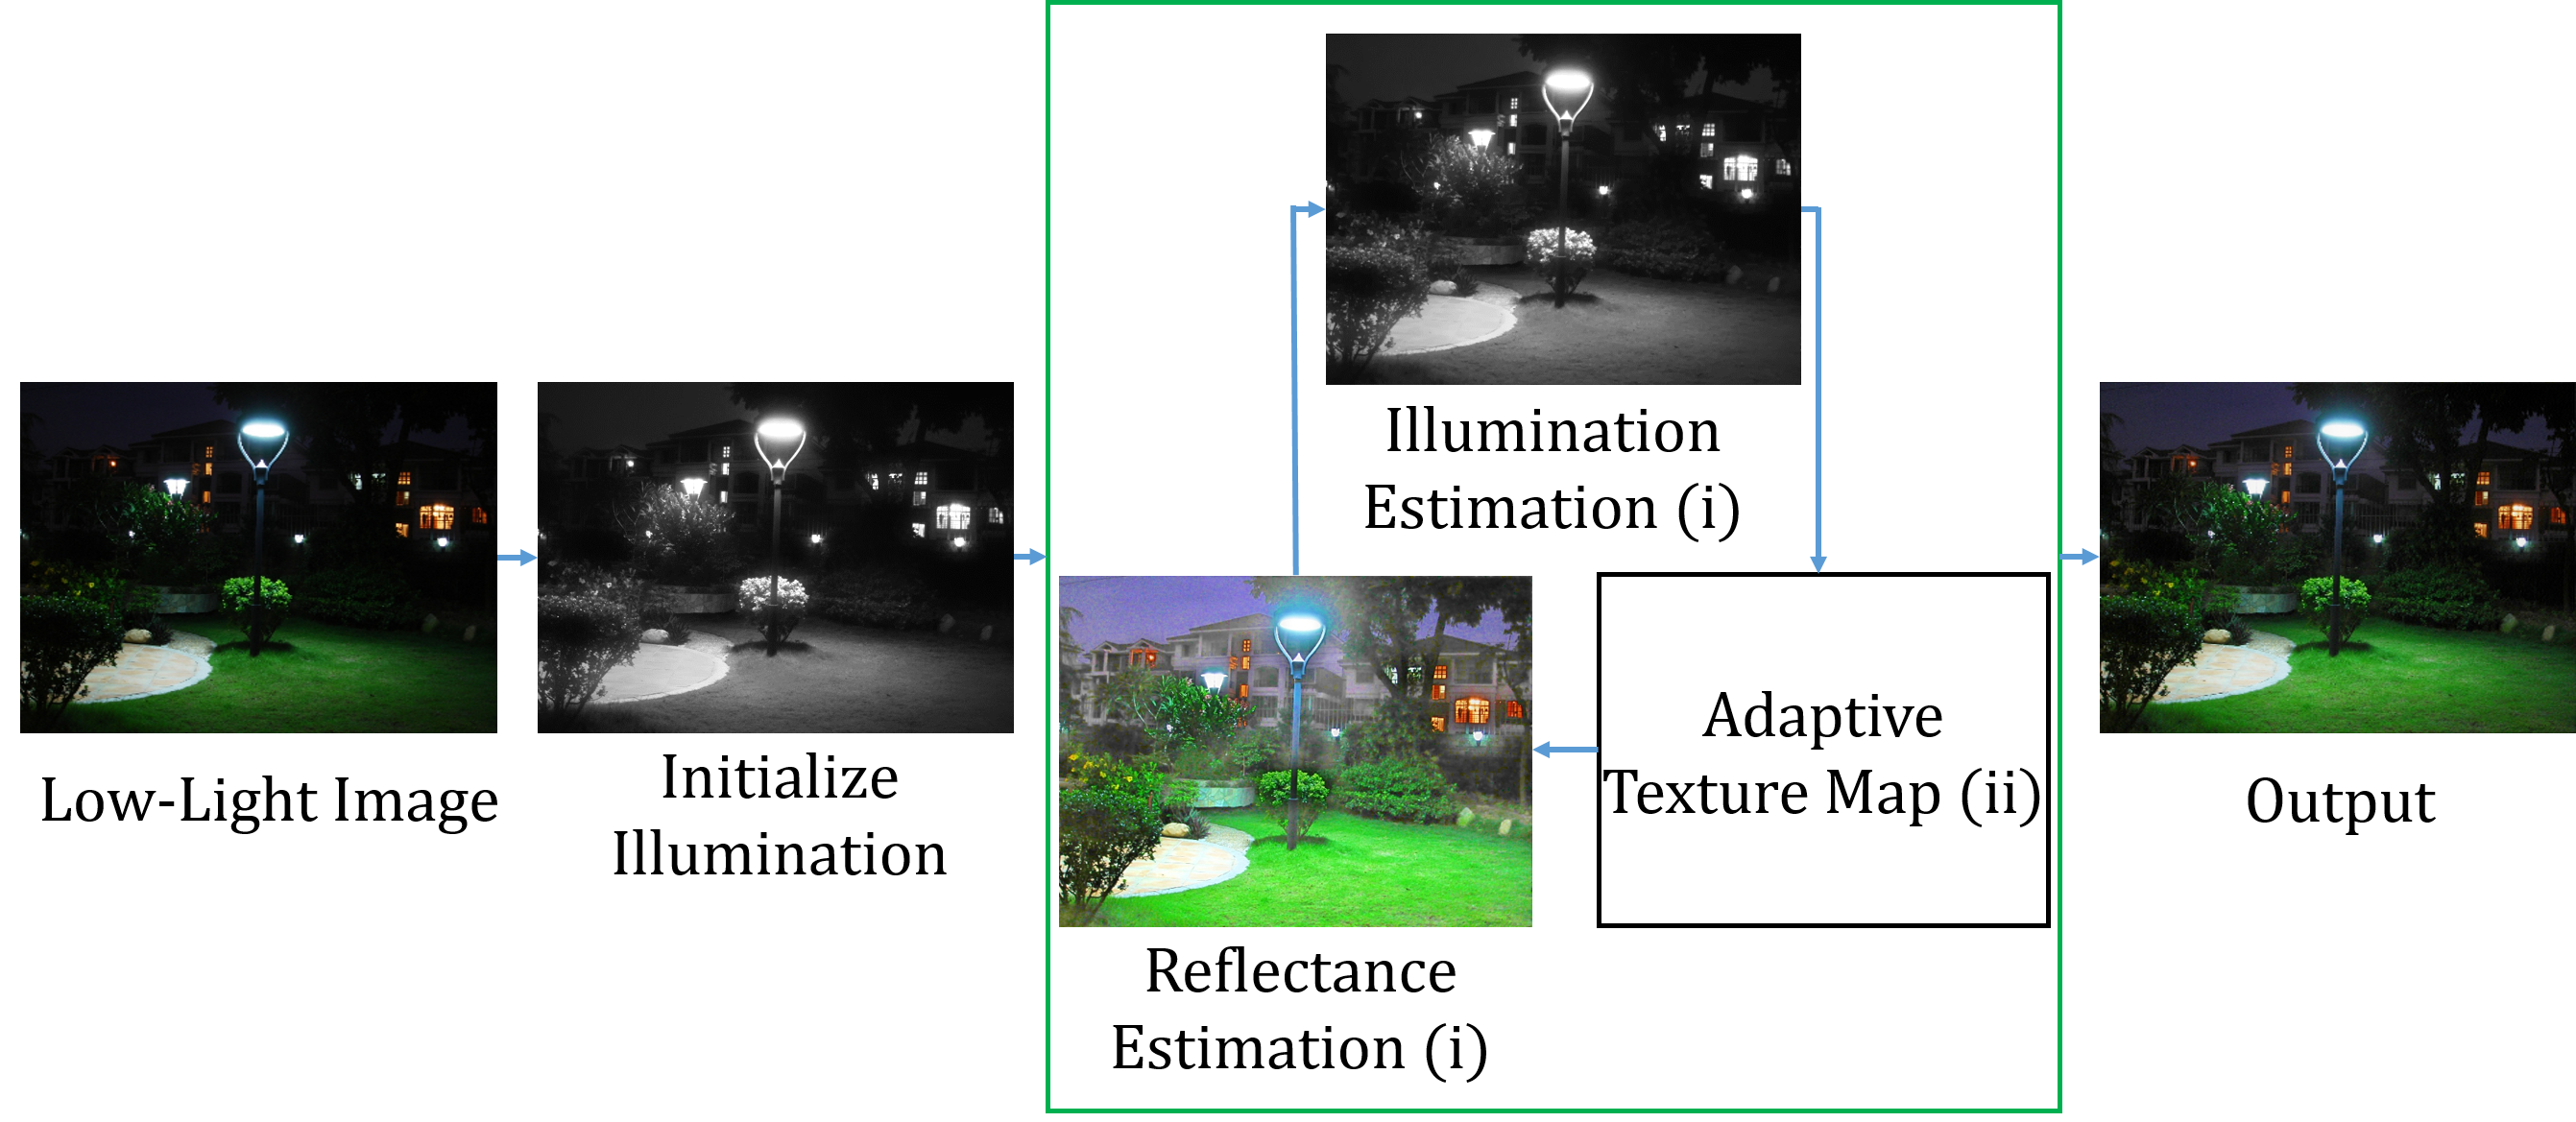
\includegraphics[width=1.0\hsize]{images/proposed/flowchart.eps}
	\caption{Flowchart of the proposed method. (i)The proposed method changes the constraint terms which further considers the characteristics for reflectance and illumination. (ii)The proposed method develop an adaptive texture map as a weight of the constraint term on reflectance which tunes the noise reduction rate according to the brightness of an observed image and texture component in reflectance.} \label{fig:proposed/flowchart}
\end{figure}
\section{Mixture L2-LP Variational Model} \label{sec:L2-LP}
The conventional methods adopt a $L_{1}$ norm to the constraint term on reflectance, but the fine details of the estimated reflectance are susceptible to be damaged. Furthermore, by adopting a $L_{2}$ norm to the constraint term on illumination, the estimated illumination loses the structure information due to over-smoothing. Therefore, the proposed method introduces $L_{2}$ and $L_{P}$ norm into the constraint terms on reflectance and illumination in a cost function. As a result, the proposed method can preserve fine textures detail as much as possible in the reflectance estimation, and keep the structure information as much as possible while avoiding the texture-copy problem in the illumination estimation. Thus, we formulate the proposed cost function of the minimization optimization problem as:
\begin{equation}
\begin{split}
	&\argmin_{R, I}{\:E(R, I)}\\
	&E(I, R) = \|R \circ I - S\|_{2}^{2} + \alpha \left \|\frac{\nabla{I}}{\frac{1}{|\Omega|}\Sigma_{\Omega}\nabla{I}+\epsilon}\right\|_{p}^{p} + \beta \|W \circ \nabla{R}\|_{2}^{2} + \gamma \|I - B\|_{2}^{2}, \label{eq:proposed/equation}
\end{split}
\end{equation}
where $\| \cdot \|_{p}$ denotes the $L_{p}$ norm constraint term $(0 \leq p \leq 2)$, and $W$ is the adaptive texture map which tunes the noise reduction rate according to the brightness of an observed image and texture component in reflectance.\par
As described in \cite{l2-lp}, a block coordinate descent method \cite{block} is used in order to find an optimal solution to the non-convex objective Eq.$(\ref{eq:proposed/equation})$. Since the $L_{p}$ norm constraint term causes non-smooth optimization, the proposed method adopts an iteratively re-weighted least square (IRLS) method \cite{iterate} and rewrite the second term in Eq.$(\ref{eq:proposed/equation})$ as:
\begin{equation}
\left \|\frac{\nabla{I}}{\frac{1}{|\Omega|}\Sigma_{\Omega}\nabla{I}+\epsilon}\right\|^{p} = \|U \circ \nabla{I}\|^{2}, \label{eq:approximation}
\end{equation}
\begin{align}
U &= \left \{
	\begin{array}{ll}
	\frac{1}{\xi^{2-p}}, 
	& \left |\frac{\nabla{I}}{\frac{1}{|\Omega|} \sum_{\Omega} \nabla{I} } \right| < \xi\\
	\frac{\left |\frac{1}{|\Omega|} \Sigma_{\Omega} \nabla{I} \right|^{2-p}}{\left |\nabla{I} \right|^{2-p}} \frac{1}{\left |\Sigma_{\Omega} \nabla{I} \right|^{2}},
	& \rm{otherwise}
	\end{array} \notag
\right.\\ 
  &= \left \{
  	\begin{array}{ll}
  	\frac{1}{\xi^{2-p}}, 
  	& \left |\frac{\nabla{I}}{\frac{1}{|\Omega|} \sum_{\Omega} \nabla{I} } \right| < \xi\\
  	\frac{1}{\left |\frac{1}{|\Omega|}\Sigma_{\Omega} \nabla{I} \right|^{p} \left |\nabla{I} \right|^{2-p}},
  	& \rm{otherwise}
  	\end{array}
\right. , \label{eq:lp_shape}
\end{align}
where $U$ is a weight matrix to approximate the $L_{0} $ norm function by using a $L_{2}$ norm format based on \cite{l0-sparse}. As can be seen in Fig.\ref{fig:nom_p/comparison}, the red curve can approximate the most sparse $L_{0}$ function. Therefore, the proposed method can remove fine textures detail and preserve meaningful salient structures in the estimated illumination. As shown in Fig.\ref{fig:nom_p/graph_norm_p}, with the decease of the value $\xi$, the $L_{p}$ norm function is getting close to the $L_{0}$ function. Therefore, as the value of $\xi$ is getting large, the more convex-like the $L_{p}$ norm function is. In addition, it is easier to optimize the cost function. In contrast, as the value of $\xi$ is getting small, the more steep the $L_{p}$ norm function is. Therefore, it is more difficult to optimize cost function.\par
Fig.\ref{fig:comparison_p} shows the effect of changing the value of $p$ in the range ($0 \leq p \leq 2$) in the estimated illumination. As the value of $p$ decreases, the estimated illumination becomes smooth and texture-less, while the estimated reflectance contains more rich textures detail. In particular, when $p=0$, some salient structure information in the estimated illumination may be lost too much, because the $L_{0}$ norm has strong sparsity. 
%----Lpノルムの概形----
\begin{figure}[tb]
\vspace{-15pt}
	\begin{minipage}[b]{0.49\hsize}
		\centering
		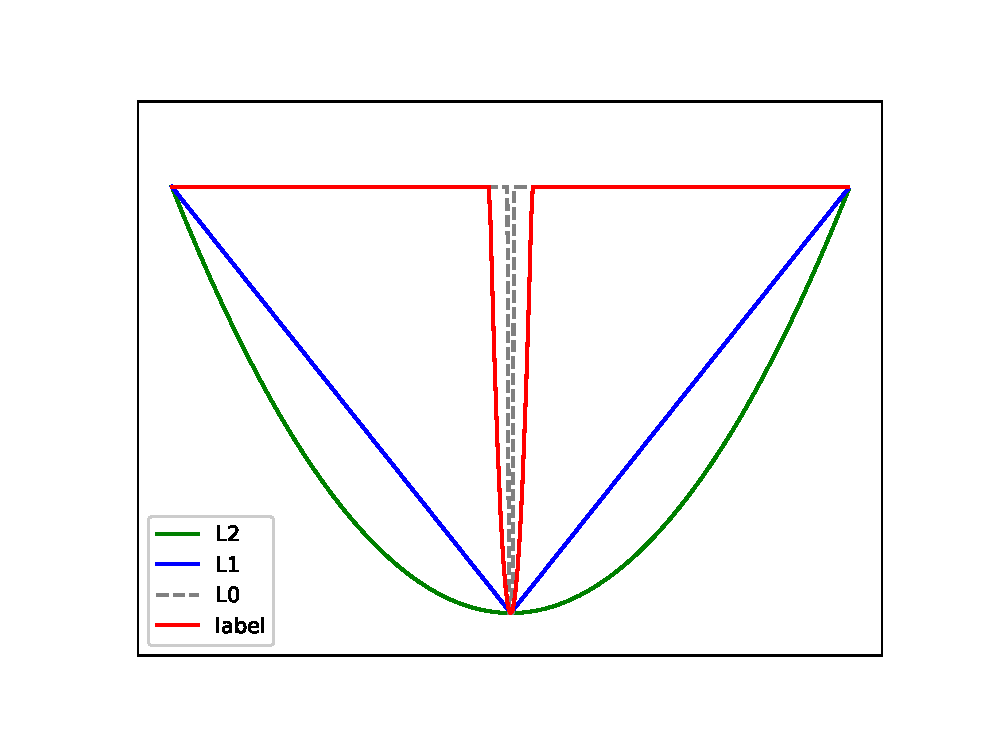
\includegraphics[width=72mm, height = 60mm]{images/norm_p/graph/graph_norm.eps}
		\subcaption{Plots of different penalty functions} \label{fig:nom_p/comparison}
	\end{minipage}
	\begin{minipage}[b]{0.49\hsize}
		\centering
		\includegraphics[width=72mm, height = 60mm]{images/norm_p/graph/graph_norm_p.eps}
		\subcaption{Plots of $L_{p}$ norm for different values $p$} \label{fig:nom_p/graph_norm_p}
	\end{minipage}
	\caption{Plots of the analysis of the $L_{p}$ norm function when $p=0$.}
	\label{fig:graph_lp}
\end{figure}
%----ノルムpによる推定比較---- %
\begin{figure}[tb]
\centering
	\begin{minipage}[b]{0.32\hsize}
	\centering
	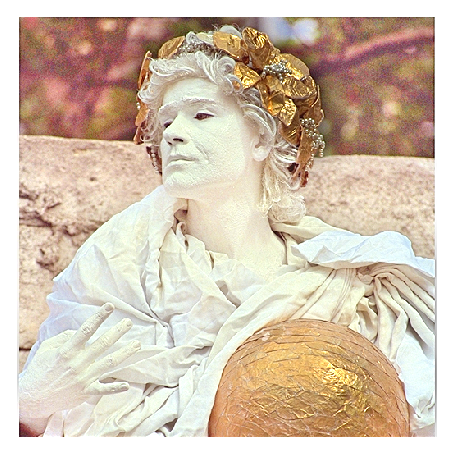
\includegraphics[width=49mm, height = 49mm]{images/norm_p/reflectance/p06.eps}
	\end{minipage}
	\begin{minipage}[b]{0.32\hsize}
	\centering
	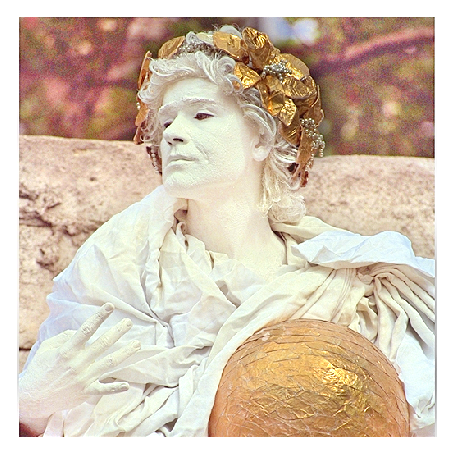
\includegraphics[width=49mm, height = 49mm]{images/norm_p/reflectance/p10.eps}
	\end{minipage}
	\begin{minipage}[b]{0.32\hsize}
	\centering
	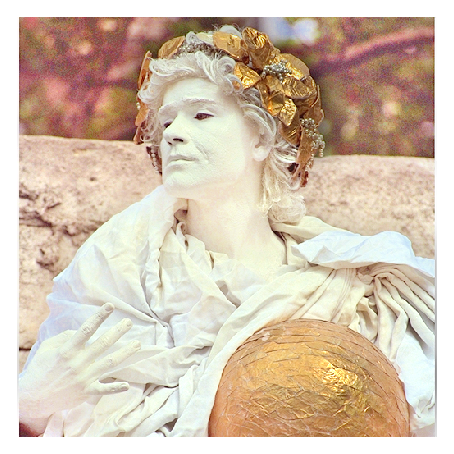
\includegraphics[width=49mm, height = 49mm]{images/norm_p/reflectance/p20.eps}
	\end{minipage}\\
	\vspace{1.5mm}
	\begin{minipage}[b]{0.32\hsize}
	\centering
	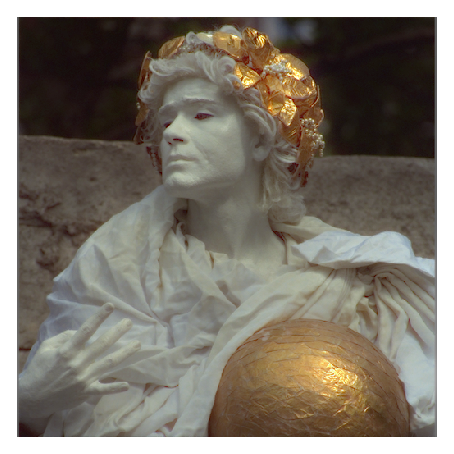
\includegraphics[width=49mm, height = 49mm]{images/norm_p/illumination/p06.eps}
	\subcaption{$p$=0.6} \label{fig. p-04}
	\end{minipage}
	\begin{minipage}[b]{0.32\hsize}
	\centering
	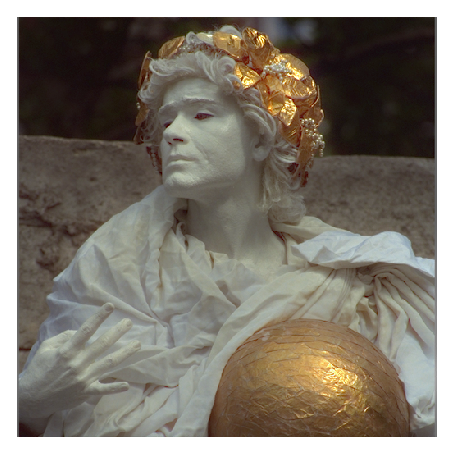
\includegraphics[width=49mm, height = 49mm]{images/norm_p/illumination/p10.eps}
	\subcaption{$p$=1.0} \label{fig. p-10}
	\end{minipage}
	\begin{minipage}[b]{0.32\hsize}
	\centering
	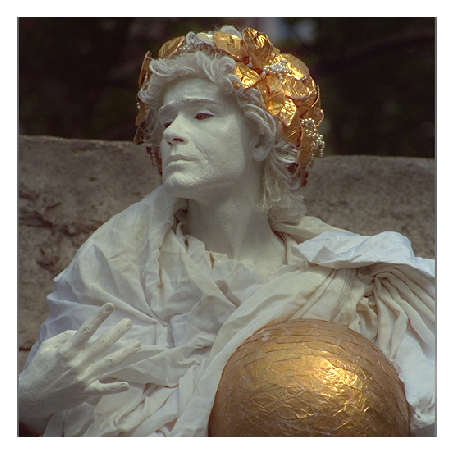
\includegraphics[width=49mm, height = 49mm]{images/norm_p/illumination/p20.eps}
	\subcaption{$p$=2.0} \label{fig. p-20}
	\end{minipage}
	\caption{Comparison of decomposition results for different values of norm $p$. ((a)-(c) top: reflectance, bottom: illumination)}
	\label{fig:comparison_p}
\end{figure}

\section{Adaptive Texture Map} \label{sec:adaptive}
This section discusses the effect of an adaptive texture map using as a weight of the constraint term on reflectance. As discussed in Sec.\ref{sec:retinex}, reflectance component contains rich details. However, when a low-light image is enhanced, noise hidden in dark regions is amplified and over-enhancement is caused in bright regions. Therefore, the constraint term on reflectance requires the weight which tunes the noise reduction rate according to the brightness of an observed image. In addition, the preferable reflectance's gradients should be smooth in homogeneous regions while should be preserved edges and textures details. Thus, when estimating reflectance, the weight which can recognize more texture regions is required so that the estimated reflectance is not damaged at texture regions. Fig.\ref{fig:adaptive/classification} shows the summary of the above discussion. Then, the adaptive texture map $W$ is set so that the third term in Eq.\ref{eq:proposed/equation} performs strong noise reduction in dark and homogeneous regions, while it performs weak noise reduction in bright and texture regions. 
Such a map $W$ is formulated as:
\begin{equation}
W_{d} = W_{B} \circ A_{d}, \label{eq:adaptive_texture}
\end{equation}
where $d$ represents horizontal ($h$) and vertical ($v$) directions, and $W_{B}$ represents an initial estimated weight map by inverting the normalized bright channel of an observed image, and $A_{d}$ represents a texture map that effectively distinguishes between homogeneous and texture regions.\par
In the same way as in \cite{activation}, given an observed low-light image, $W_{B}$ should selectively assigns different values to dark and bright regions according to BCP since the estimated bright channel contains small values in dark regions and vice versa. Thus, $W_{B}$ is given as:
\begin{equation}
W_{B} = 1.0 - \max_{c \in \{r, g, b\}}S^{c}. \label{eq:adaptive/initial_weight}
\end{equation}
Fig.\ref{fig:adaptive/wb} shows the image of $W_{B}$. Since larger weight values are assigned in dark regions, $W_{B}$ performs a stronger noise reduction. In contrast, a weaker noise reduction is performed in bright regions by $W_{B}$.\par
Moreover, the texture map $A_{d}$ is set as the inverse of the $a_{r}$-th power of the absolute value of a mean local variation (MLV) \cite{jiep}, so that it can significantly distinguish between homogeneous regions and texture regions:
\begin{equation}
A_{d} = \frac{1}{\left |\frac{1}{|\Omega|}\sum_{\Omega}\nabla_{d}{R} \right|^{a_{r}} + \epsilon}, \label{eq: mlv}
\end{equation}
where $a_{r} (0 \leq a_{r} \leq 1)$ is an exponential parameter to adjust the awareness of textures detail for reflectance. 
As shown in Fig.\ref{fig:mlv_normal} and \ref{fig:mlv_pow}, when $a_{r}=1.0$, the texture map $A_{d}$ extracts salient edges but little texture component. In contrast, when $a_{r}=0.5$, the texture map extracts both salient edges and rich texture component, but the map amplifies details in flat and homogeneous regions. Therefore, the exponential parameter $a_{r}$ should be set small in salient edges and textures details, and set large in flat and homogeneous regions, so that
\begin{equation}
a_{r} = 1.0 - |\nabla_{d}{R}|\exp(1.0 - |\nabla_{d}{R}|). \label{eq:adaptive/parameter}
\end{equation}
Fig.\ref{fig:mlv_prop} shows the proposed MLV of reflectance. The regions of edges and textures detail are getting revealed and the flat and homogeneous regions are controlled. Therefore, using the texture map, $W$ performs the weaker noise reduction in both edges and texture regions, while performs the stronger noise reduction in homogeneous regions.\par
The discussion centers on the effectiveness of the adaptive texture map using Fig.\ref{fig:adaptive/effectiveness}.
As shown in the yellow and green squares, the estimated reflectance with $W$ can suppress noise amplification in dark regions and over-enhancement in bright regions more than without $W$. This is because $W_{B}$ can effectively assign different values between dark and bright regions. 
Next, in order to confirm the effectiveness of the texture map $A_{d}$, the edge magnitude in the red square is calculated:
\begin{equation}
M(h, v) = \sqrt{G_{h} ^{2}+ G_{v}^{2}}, \label{eq:maginitude}
\end{equation}
where $G_{h}$ and $G_{v}$ represent the horizontal and vertical gradient images, respectively. Fig.\ref{fig:adaptive/edge_magnitude} shows the plots of average v-axis edge magnitude. It can be seen that the average gradient magnitude with $W$ has larger values and the values fluctuate more rapidly than the ones without $W$. Therefore, the texture map $A_{d}$ contributes to the awareness of textures in the estimated reflectance.
% ----Classificationの図----%
\begin{figure}[tb]
	\centering
	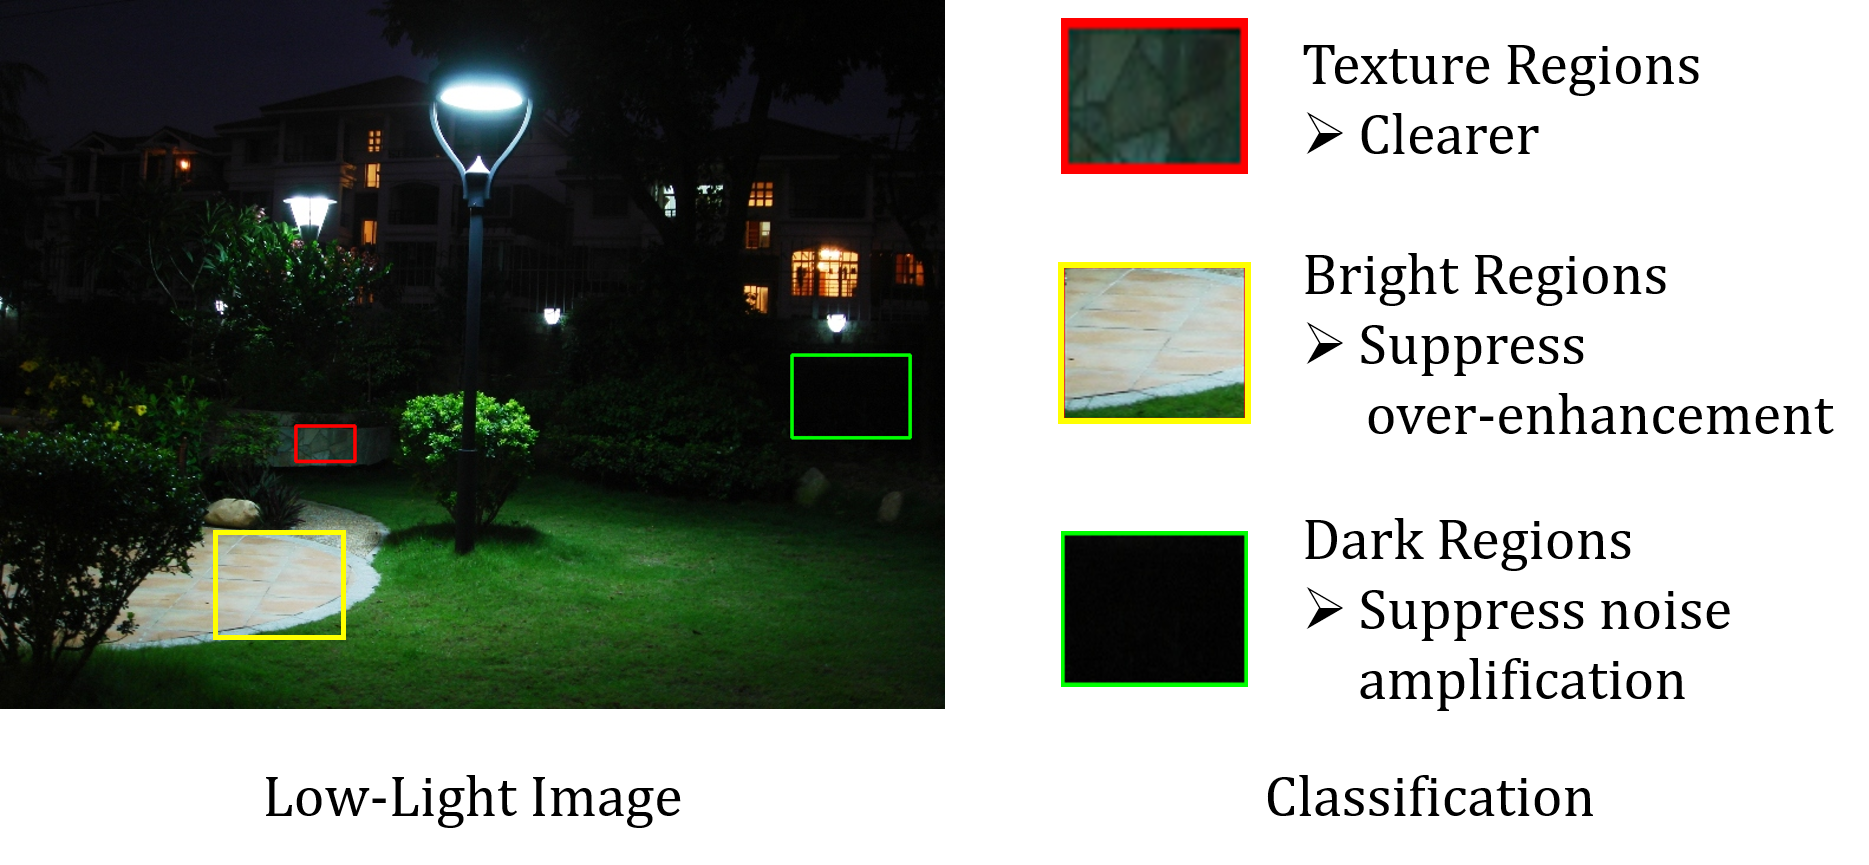
\includegraphics[width=0.8\hsize]{images/adaptive/classification.eps}
	\caption{Classification of regions where the adaptive texture map has an impact on.} \label{fig:adaptive/classification}
\end{figure}
% ----Weight of BCPの図----%
\begin{figure}[htbp]
	\centering
	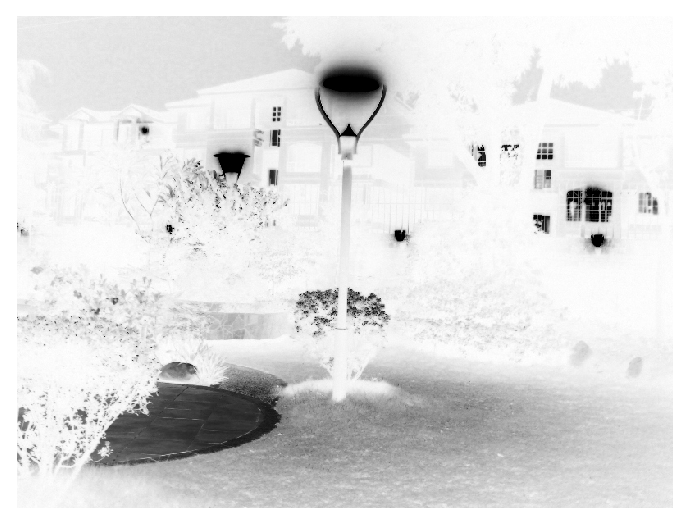
\includegraphics[width=60mm, height=48mm]{images/adaptive/wb.eps}
	\caption{The image of $W_{B}$. $W_{B}$ contains larger values in dark regions, while contains smaller values in bright regions, while contains larger values in dark regions.} \label{fig:adaptive/wb}
\end{figure}
% ----Texture Mapの図----%
%\begin{figure}[tb]
%\centering
%\begin{minipage}[b]{0.32\hsize}
%\centering
%\includegraphics[width=48mm, height=36mm]{images/noise/mlv_10.eps}
%\subcaption{MLV ($a_{r}=1.0$)} \label{fig:mlv_normal}
%\end{minipage}
%\begin{minipage}[b]{0.32\hsize}
%\centering
%\includegraphics[width=48mm, height=36mm]{images/noise/mlv_05.eps}
%\subcaption{MLV ($a_{r}=0.5$)} \label{fig:mlv_pow}
%\end{minipage}
%\begin{minipage}[b]{0.32\hsize}
%\centering
%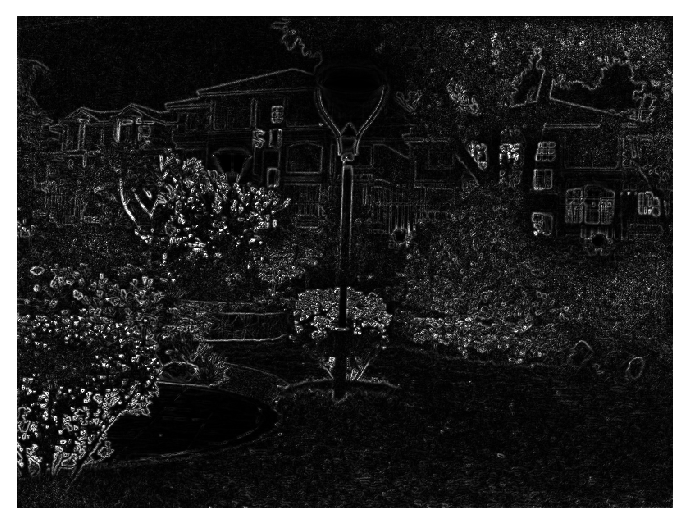
\includegraphics[width=48mm, height=36mm]{images/noise/mlv_prop.eps}
%\subcaption{MLV (the proposed $a_{r}$)} \label{fig:mlv_prop}
%\end{minipage}
%\caption{Comparison of MLV results for different values of $a_{r}$. The proposed $a_{r}$ contributes to distinguish between %regions which should reveal and regions which should control.}
%\label{fig:mlv_change}
%\end{figure}
% ----Texture Mapの図----%
\begin{figure}[t]
	\centering
	\begin{minipage}[b]{0.49\hsize}
		\centering
		\includegraphics[width=60mm, height=48mm]{images/noise/mlv_10.eps}
		\subcaption{MLV ($a_{r}=1.0$)} \label{fig:mlv_normal}
	\end{minipage}
	\begin{minipage}[b]{0.49\hsize}
		\centering
		\includegraphics[width=60mm, height=48mm]{images/noise/mlv_05.eps}
		\subcaption{MLV ($a_{r}=0.5$)} \label{fig:mlv_pow}
	\end{minipage}
	\begin{minipage}[b]{0.49\hsize}
		\centering
		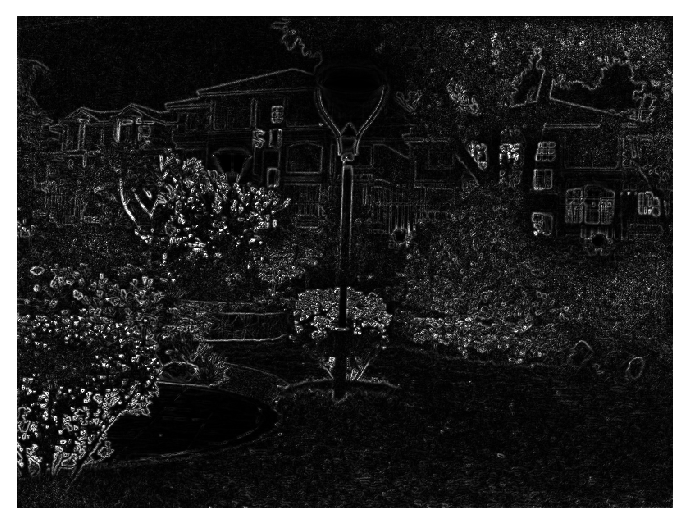
\includegraphics[width=60mm, height=48mm]{images/noise/mlv_prop.eps}
		\subcaption{MLV (the proposed $a_{r}$)} \label{fig:mlv_prop}
	\end{minipage}
	\caption{Comparison of MLV results for different values of $a_{r}$. The proposed $a_{r}$ contributes to distinguish between regions which should be revealed and regions which should be constrained.}
	\label{fig:mlv_change}
\end{figure}
% ----Texture Mapの抑制図----%
\begin{figure}[tb]
	\centering
	\begin{minipage}[b]{0.49\hsize}
		\centering
		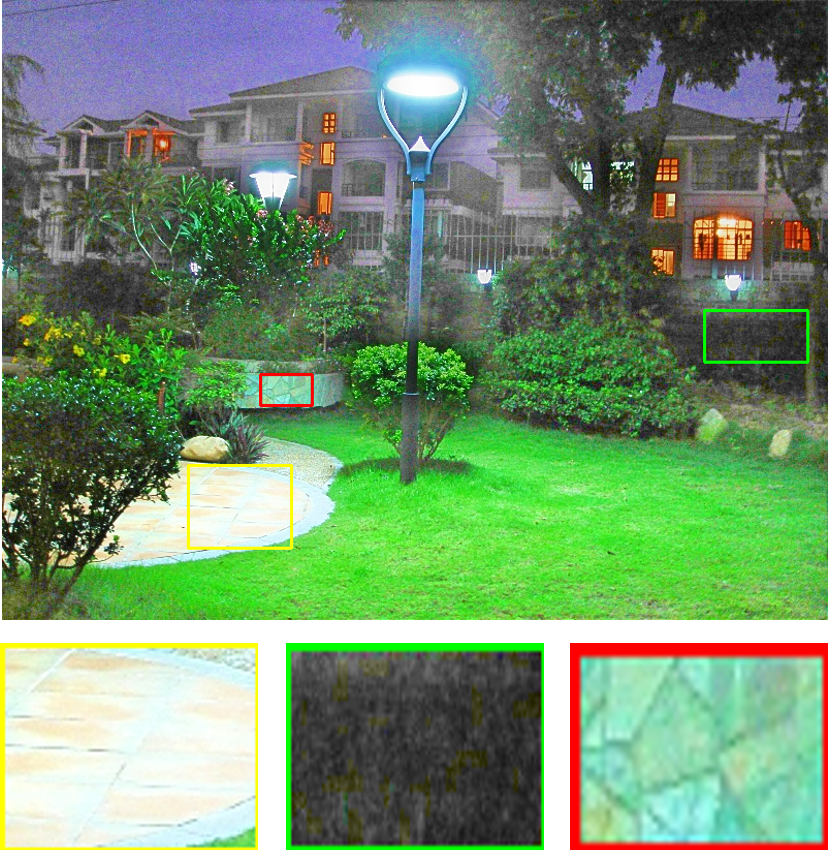
\includegraphics[width=60mm, height=60mm]{images/adaptive/without.eps}
		\subcaption{Reflectance w/o $W$} \label{fig:wo}
	\end{minipage}
	\begin{minipage}[b]{0.49\hsize}
		\centering
		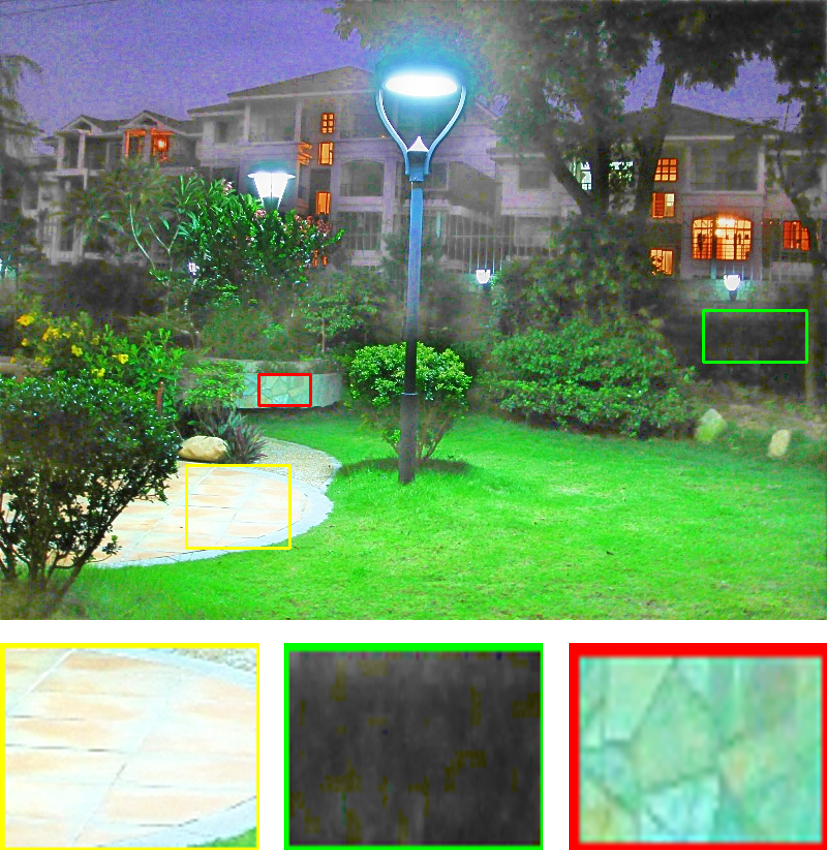
\includegraphics[width=60mm, height=60mm]{images/adaptive/with.eps}
		\subcaption{Reflectance with $W$} \label{fig:w}
	\end{minipage}
	\caption{Comparison of reflectance results. (a) the estimated reflectance without $W$; (b) the estimated reflectance with $W$.}
	\label{fig:adaptive/effectiveness}
\end{figure}
% ----Edge Magnitudeの図----%
\begin{figure}[tb]
	\centering
	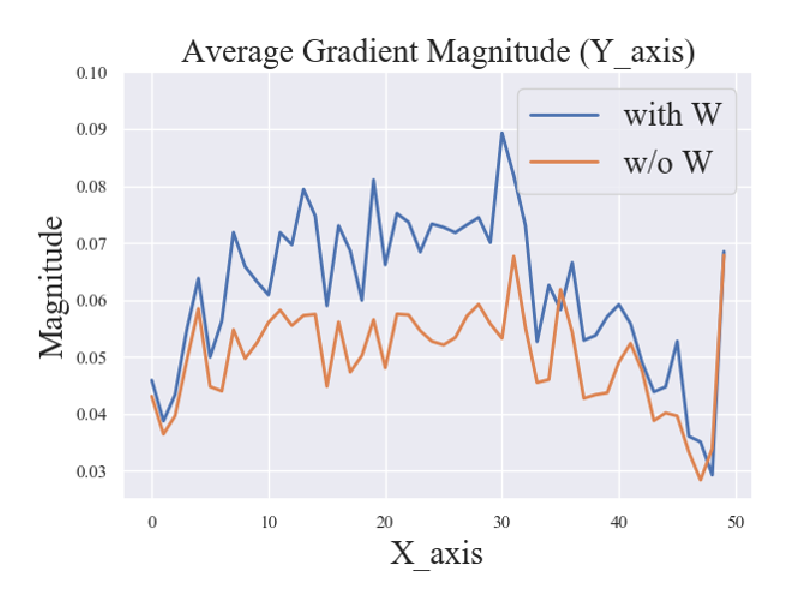
\includegraphics[width=0.8\hsize]{images/adaptive/graph_edge.eps}
	\caption{Plots of the average edge magnitude.} \label{fig:adaptive/edge_magnitude}
\end{figure}

\section{Solution} \label{sec:solution}
The optimization problem (\ref{eq:proposed/equation}) can be solved by iteratively updating sub-problems for reflectance and illumination. In particular, for the $k$-th iteration of sub-problems:
\begin{enumerate}
\renewcommand{\labelenumi}{\arabic{enumi}).}
\item \textbf{$\boldmath{I}$ sub-problem:} Collecting the terms related to $I$ leads to the following sub-problem in (\ref{eq:proposed/equation}):
\begin{equation}
I_{k} = \argmin_{I}\|R_{k-1} \circ I - S\|_{2}^{2} + \alpha\|U \circ \nabla{I}\|_{2}^{2} 
+\lambda \|I - B\|_{2}^{2}. \label{eq:i_subproblem}
\end{equation}
The sub-problem (\ref{eq:i_subproblem}) results in a classic least square problem:
\begin{equation}
i_{k} = \argmin_{i} \|r_{k-1} i - s\|_{2}^{2} + \alpha\|uDi\|_{2}^{2} + \lambda \|i - b\|_{2}^{2}, \label{eq:classic_i_subproblem}
\end{equation}
where $i$ is the vectorized format of $I$ and $D$ contains $D_{h}$ and $D_{v}$, which are the Toeplitz matrices obtained from the discrete gradient operators with forward difference.
The same notation is used for other matrices (r, s, b corresponds to R, S, and B, respectively). By differentiating the function (\ref{eq:classic_i_subproblem}) with respect to $i$, and setting the derivative to $0$, we have the following solution:
\begin{equation}
i_{k+1} = (r_{k-1}r_{k-1}^{T} + \alpha D^{T}uD + \lambda{1})^{-1} (r_{k-1}^{T}s + \lambda{b}). \label{eq: i_solution}
\end{equation}
Then, the obtained $i_{k}$ is reformulated into matrix format $I_{k}$.
\item \textbf{$R$ sub-problem:} After acquiring $I_{k}$ from the above solution, the sub-problem in  (\ref{eq:proposed/equation}) related to $R$ becomes similar to that of $I$:
\begin{equation}
R_{k} = \argmin_{R}\|R \circ I_{k} - S\|_{2}^{2} + \beta\|W \circ \nabla{R}\|_{2}^{2}. \label{eq: r_subproblem}
\end{equation}
In the same way as in the former derivation, the solution of $R$ is provided as follows:
\begin{equation}
r_{k} = \argmin_{r} \|ri_{k} - s\|_{2}^{2} + \beta\|wDr\|_{2}^{2}, \label{eq:classic_r_subproblem}
\end{equation}
\begin{equation}
r_{k} = (i_{k}i_{k}^{T} + \beta D^{T}wD)^{-1} (i_{k}^{T}s). \label{eq: solution_r_subproblem}
\end{equation}
Similarly, the obtained $r_{k}$ is reformulated into matrix format $R_{k}$.
\end{enumerate}
The values of $I$ and $R$ are updated until $\|I_{k}-I_{k-1}\|/\|I_{k-1}\| \leq \varepsilon$ and $\|R_{k}-R_{k-1}\|/\|R_{k-1}\| \leq \varepsilon$ are simultaneously satisfied. After the estimation of  reflectance and illumination, a Gamma correction operation is adopted to adjust illumination. Therefore, the final enhanced image is given as $ S_{enhanced} = R \circ I^{\frac{1}{\gamma^{'}}}, \label{eq_final}$ where the empirical parameter $\gamma^{'}$ is set as 2.2. To preserve color information, the Gamma correction is performed in the HSV-color space.
Fig.\ref{fig:proposed/output} shows the result of the proposed method. The proposed method can smooth illumination as much as possible while keeping the meaningful structure information in the illumination estimation, and clarify fine textures detail as much as possible while suppressing noise amplification in dark regions and over-enhancement in bright regions in the reflectance estimation. Therefore, we can see that the proposed method naturally enhances low-light images.
%----提案手法の結果の図---- %
\begin{figure}[tb]
\centering
	\begin{minipage}[b]{0.49\hsize}
		\centering
		\includegraphics[width=62.5mm]{images/proposed/input.eps}
		\subcaption{Low-Light Image} \label{fig:proposed/input}
	\end{minipage}
	\begin{minipage}[b]{0.49\hsize}
		\centering
		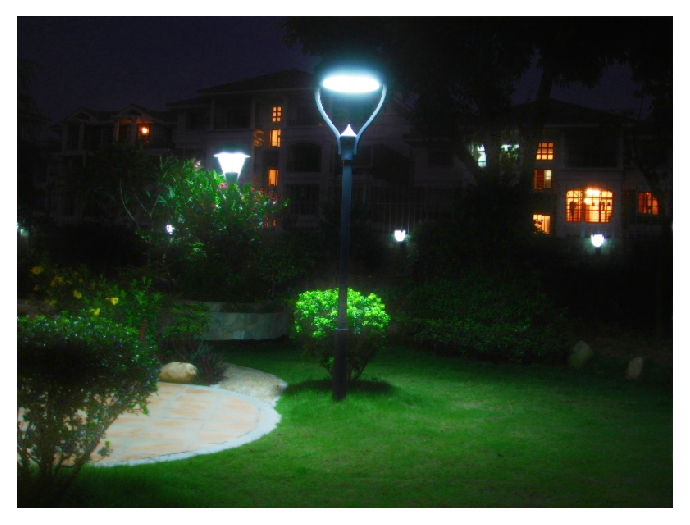
\includegraphics[width=62.5mm]{images/proposed/illumination.eps}
		\subcaption{Illumination} \label{fig:proposed/illumination}
	\end{minipage}
	\begin{minipage}[b]{0.49\hsize}
		\centering
		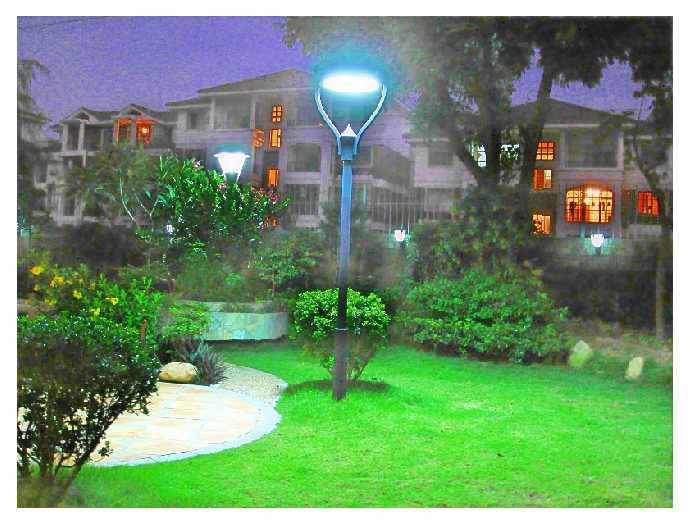
\includegraphics[width=62.5mm]{images/proposed/reflectance.eps}
		\subcaption{Reflectance} \label{fig:proposed/reflectance}
	\end{minipage}
	\begin{minipage}[b]{0.49\hsize}
		\centering
		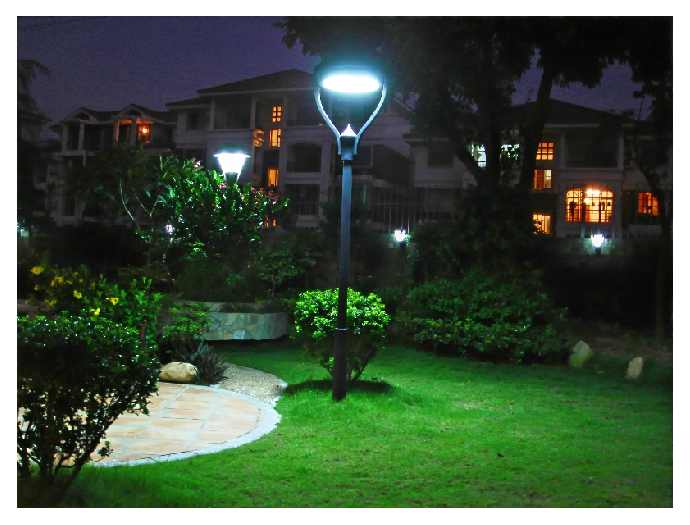
\includegraphics[width=62.5mm]{images/proposed/output.eps}
		\subcaption{Enhanced Image} \label{fig:proposed/enhanced}
	\end{minipage}
	\caption{The results of the proposed method.}
	\label{fig:proposed/output}
\end{figure}